\pagebreak
\subsection{Armature Inductance}%\label{put a label here and uncomment}
\textbf{Name: Group 510}\\
\textbf{Date: 30/09 - 2015}

\subsubsection{Purpose}
The purpose of the test is to determine the Armature inductance \si{L_a} of the motor.

\subsubsection{Setup}
\begin{figure}[H]
  \centering
	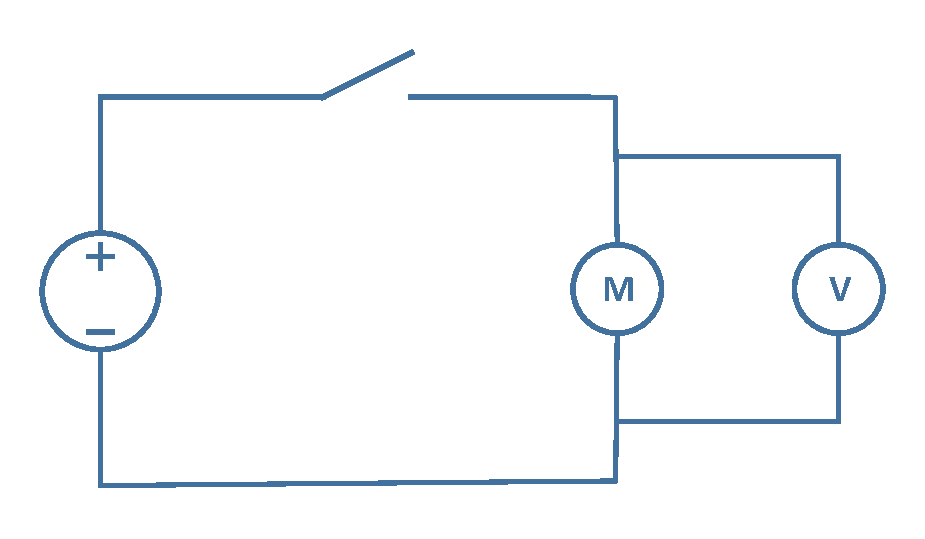
\includegraphics[scale=0.5]{figures/MotorTest2.pdf}
	\caption{Setup diagram}
\end{figure}

\subsubsection{List of Equipment}

\begin{table}[H]
\begin{tabular}{|l|l|p{4cm}|}
\hline%--------------------------------------------------------------------------------
  \textbf{Instrument}                    &  \textbf{AAU-no.}  &  \textbf{Type}       \\
\hline%--------------------------------------------------------------------------------
  Power Supply ($0 - 32$ V) ($0 - 10$ A) &  77076             &  Ea - ps 7032 - 100  \\
\hline%--------------------------------------------------------------------------------
  AC/DC Current Clamp (Output: 100 mV/A) &  78550             &  FLUKE i30s          \\
\hline%--------------------------------------------------------------------------------
  Oscilloscope                           &  64672             &  Agilent DSO6034A    \\
\hline%--------------------------------------------------------------------------------
  Clamp for fixing the motor             &  03039             &                      \\
\hline%--------------------------------------------------------------------------------
\end{tabular}
\end{table}

\subsubsection{Procedure}

\begin{enumerate}
  \item Fix the motor shaft so it can not turn.
  \item Start with the power supply disconnected and turn on the oscilloscope.
  \item On the oscilloscope press the "trigger mode"-key choose the "normal"-option and push the "single"-key.
  \item To prevent false triggering on the oscilloscope, set the trigger value to $113$ mV.
  \item To supply the motor a pulse of $5$ V, adjust the power supply to $5$ V and connect it.
  \item Connect a USB-drive to the oscilloscope and press the save key to extract the data.
\end{enumerate}

\subsubsection{Results}

\begin{figure}[H]
  \centering
 	%Trim margins @:   left        bottom       right       top
 	\adjustbox{ trim = {.15\width} {.30\height} {.15\width} {.30\height}, clip }
  {
    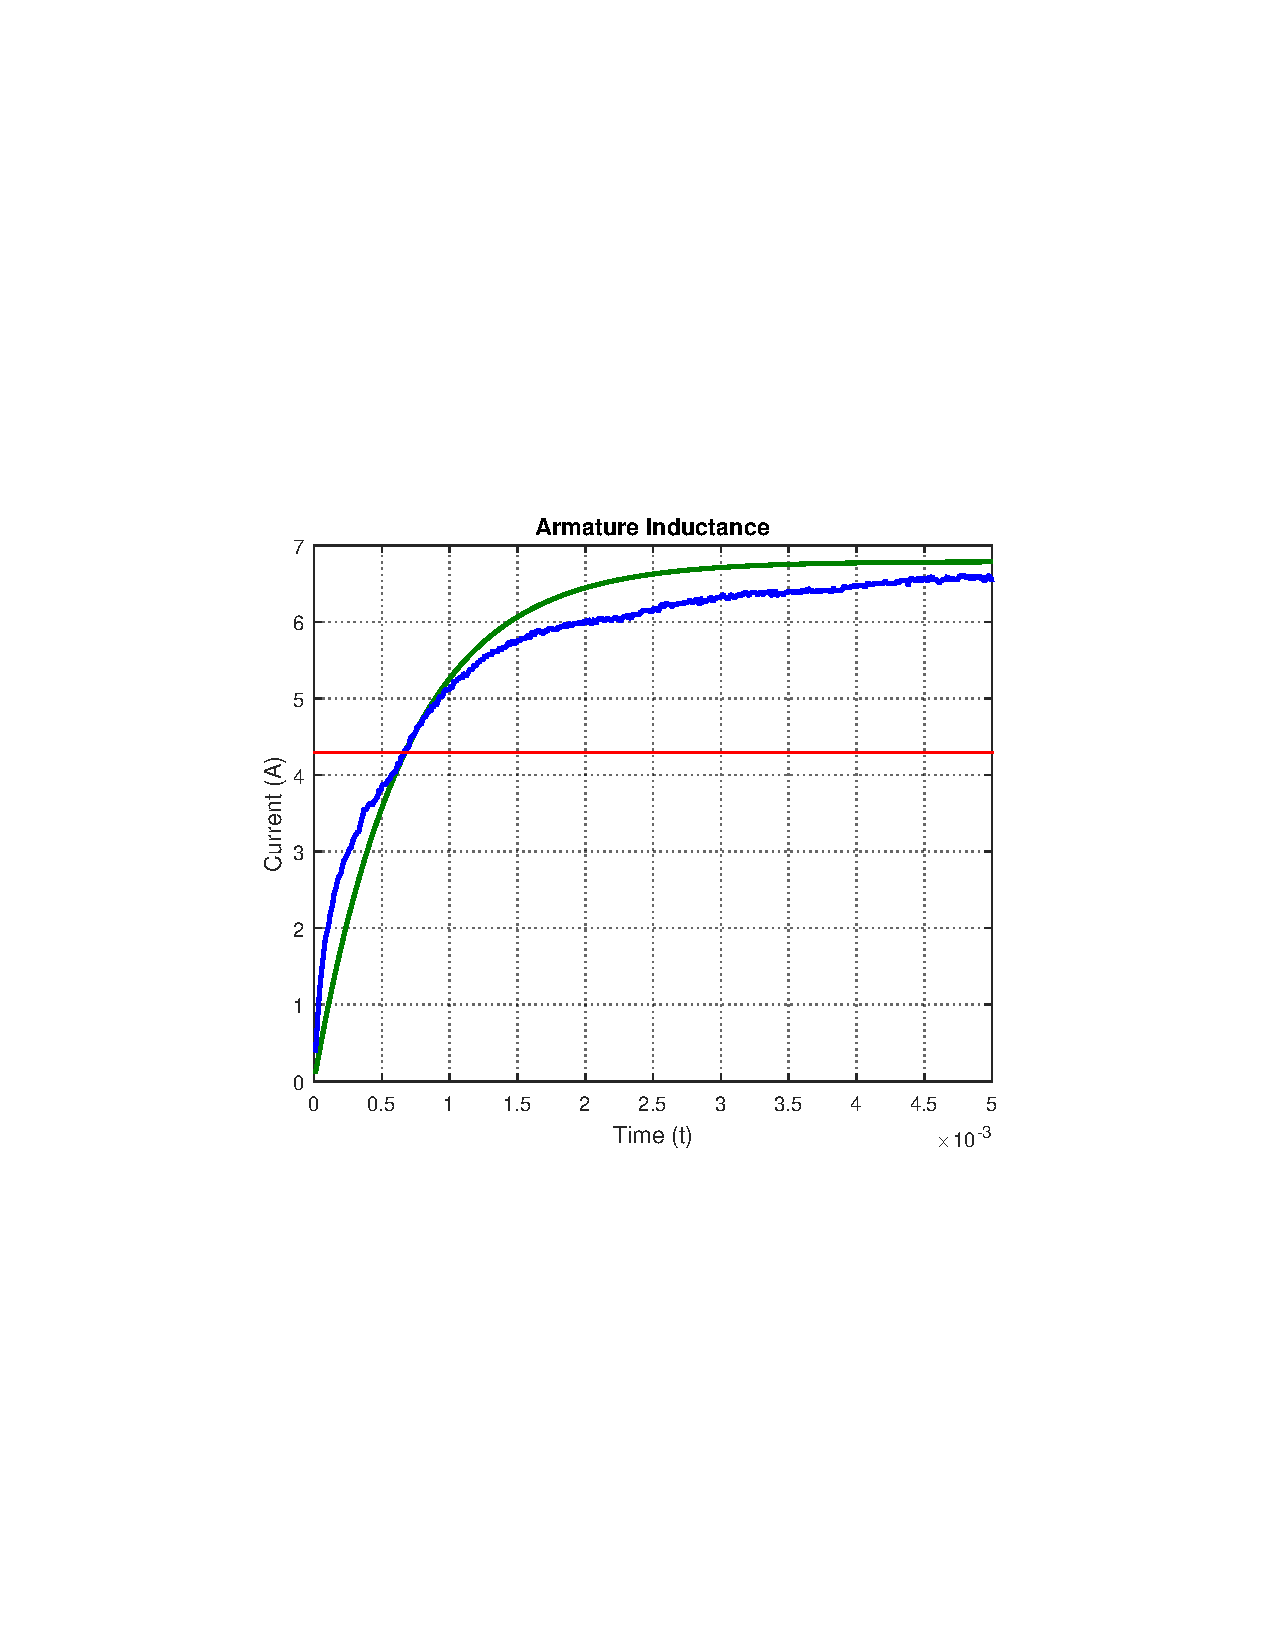
\includegraphics[width=\textwidth]{figures/armatureInductance.pdf}
  }
	\caption{A plot of a current step response of the motor, where the blue line is data, the green line is the ideal step response and the red line is the time constant}
	\label{armatureInductance}
\end{figure}

The armature inductance, \si{L_a}, is calculated from the time constant given by:
\begin{flalign}
  \eq{\tau} {\frac{L_a}{R_a}}\unit{s}\nonumber
\end{flalign}
\hspace{6mm} Where:\\
\begin{tabular}{p{1cm}ll}
  & \si{\tau} & is the time constant \unit{s}       \\
  & \si{L_a}  & is the armature inductance \unit{H} \\
  & \si{R_a}  & is the armature resistance \unit{\Omega} \\
\end{tabular}

\si{R_a} is know from the previous test, \textit{Armature Resistance}, where it was found to \si{0,178 \Omega}. $\tau$ is the time at which the current reaches \si{63,2\%} of the value at steady state. This value of $\tau$ is found by use of \figref{armatureInductance} and located in the data set:
%
\begin{flalign}
  \eq{\tau}{0,67 \cdot 10^{-3}}\unit{s}\nonumber
\end{flalign}
%
From this we get the armature inductance:
%
\begin{flalign}
  \eq{L_a}{\tau \cdot R_a}\unit{H}\nonumber\\
  \eq{L_a} {0,67 \cdot 10^{-3} \cdot 0,178}\unit{H}\nonumber\\
  \eq{L_a}{119,26}\unit{\mu H}\nonumber
\end{flalign}